\section{Results \label{sec:results}}

\begin{table}\footnotesize
\begin{center}
  \caption{Expected background event yields and observed numbers of events in data for $35.9\fbinv$. The expected number of signal events for 
the \cPZpr-2HDM model with \mz = 1000~\GeV (\maz = 300~\GeV), scaled to the nominal cross section, is also reported. 
}
\begin{tabular}{l r}
  \hline\hline
Process         & Yields          \\
\hline
Z+jets              &$ 303.9\pm6.8 $       \\
Single Top       &$29.2\pm2.2 $         \\
\ttbar          &$ 271.7\pm7.1 $        \\
W+jets          &$ 126.1\pm7.2 $            \\
SM H             &$ 29.0\pm0.2 $        \\
Diboson         &$ 27.0\pm3.1  $       \\
%Multijets       & ????  \\
\hline
Total background        &$ 786.7\pm12.8 $       \\
\hline \hline
\cPZpr-2HDM \mz = 1000~\GeV (\maz = 300~\GeV)        &$ 69.8\pm0.6 $       \\
%\cPZpr-2HDM \mz = 1700~\GeV (\maz = 300~\GeV)        &$ ????\pm ???? $     \\

%\cPZpr-Baryonic \mz = 100~\GeV (\mdm = 1~\GeV)        &$ ????\pm ???? $       \\
%\cPZpr-Baryonic \mz = 1000~\GeV(\mdm = 1~\GeV)        &$ ????\pm ???? $     \\
Data            & -         \\
\hline\hline
  \end{tabular}
\label{tab:eventYieldTable}
\end{center}
\end{table}



Table \ref{tab:eventYieldTable} shows the 
SR expected yields for each background and one signal mass hypothesis for the \cPZpr-2HDM model, along with the 
size of the statistical uncertainties.


Since no excess of events has been observed over the SM background expectation in the SR, the results of this search are interpreted in terms of an upper limit on the production cross 
section of DM candidates in association with a Higgs boson. 
The upper limits are calculated at 95\% confidence level (CL) using a modified frequentist method (CL$_s$) \cite{yellowReport, bib:CLS1, bib:CLS2} computed with an asymptotic approximation \cite{bib:CLS3}. 
A profile likelihood ratio is used as the test statistic in which systematic uncertainties are modeled as nuisance parameters.

\begin{figure}[htbp]
  \centering
  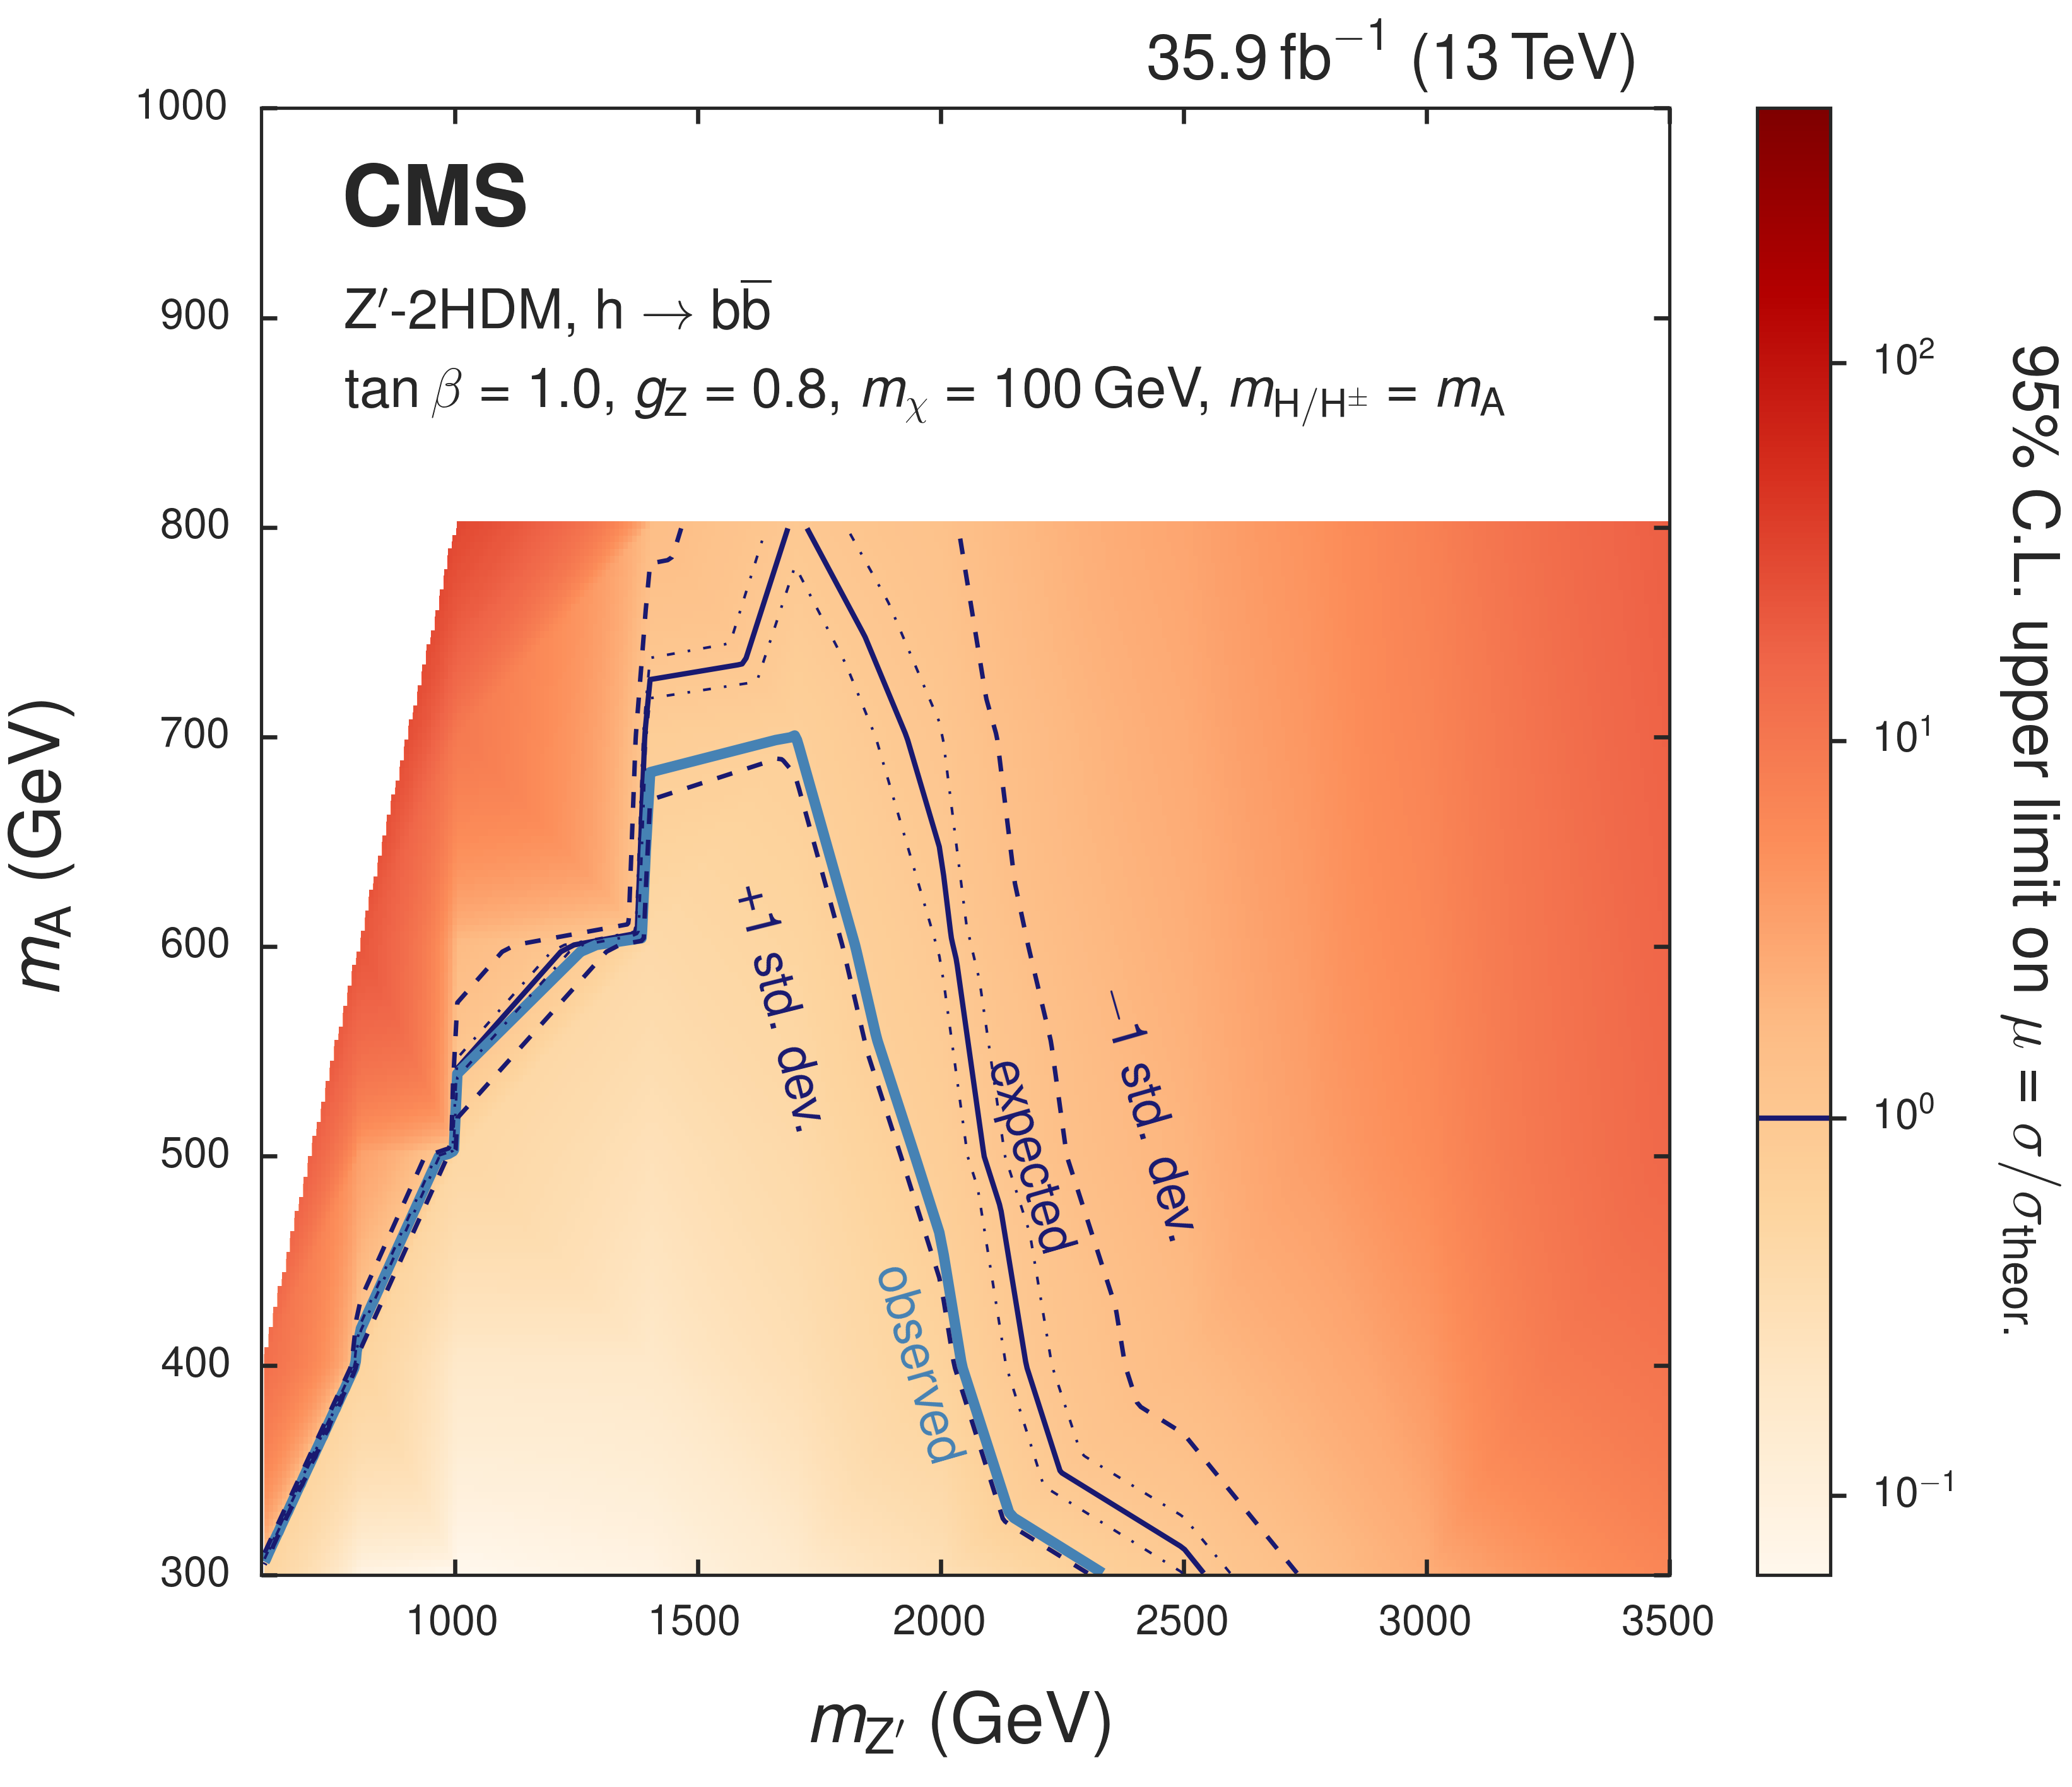
\includegraphics[width=0.475\textwidth]{figures/limits/limits_2hdm2d.png}
  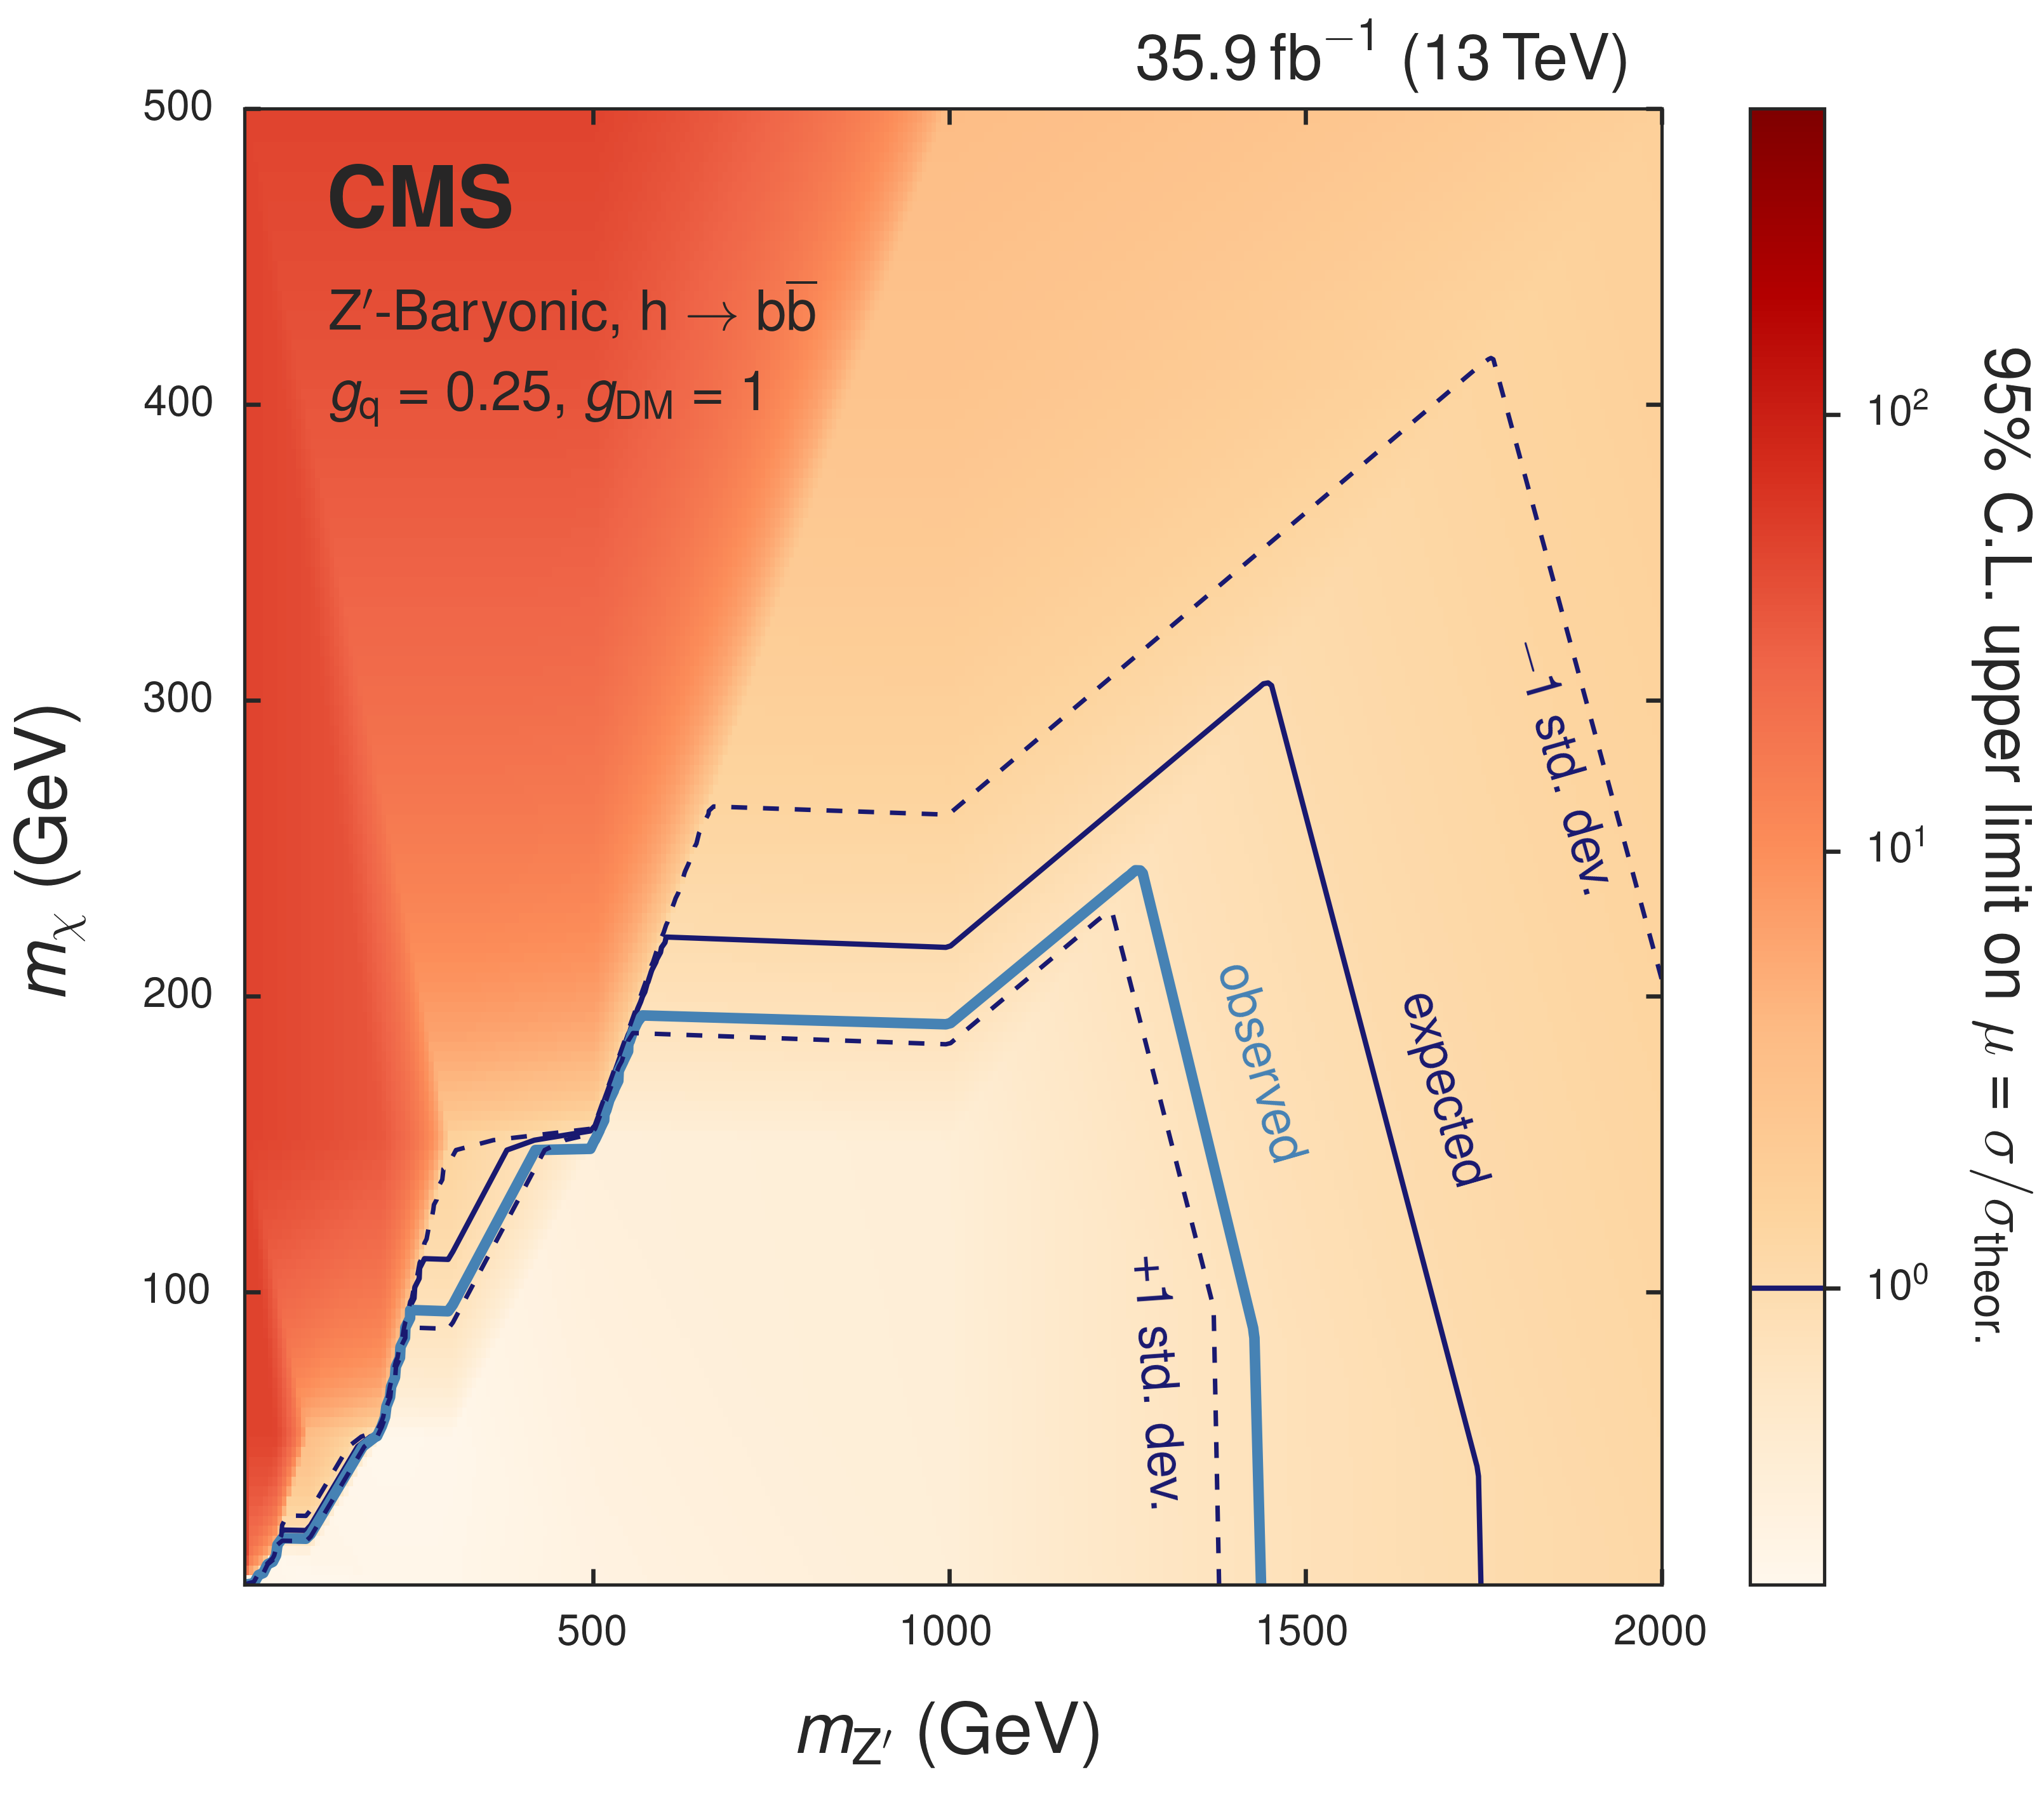
\includegraphics[width=0.475\textwidth]{figures/limits/limits_barzp2d.png}
  \caption{Upper limits on the signal strength modified for the 2HDM model (left) and Z'-Baryonic model (right).}
  \label{fig:limits}
\end{figure}

Figure~\ref{fig:limits} shows the expected and observed exclusions as a function of $m_{Z'}$ and $m_{A^0}$ for the \cPZpr-2HDM model and as a function of $m_{Z'}$ and $m_{\chi}$ for the 
baryonic $\cPZpr_{B}$ model. The excluded mass for $\mathrm{Z}'$ for $m_{A^0}=300$\,GeV is ???, while the largest excluded $\mathrm{Z}'$ mass in the $\mathrm{Z}'$-Baryonic model is ???. %Other assumptions are on $tan\beta = 1.0$, $g_{Z'} = 0.8$, and $m_{\chi} = 100$ GeV for the 2HDM, while for the Baryonic Z' model coupligs are assumed to be $g_{q} = 0.25, g_{\chi}=1~GeV$.

Results on the associated production of DM particles with Higgs boson decaying in a b-quark pair have been presented. Limits on the production cross section predicted by the \cPZpr-2HDM and the baryonic $\cPZpr_{B}$ model are set and they constitute the most stringent limits on the parameters in these models so far. 
